\documentclass[preprint,12pt,authoryear]{elsarticle}
\usepackage[utf8]{inputenc}
\usepackage[T1]{fontenc}
\usepackage{amsmath,amssymb}
\usepackage{graphicx}
\usepackage{booktabs}
\usepackage{multirow}
\usepackage{xcolor}
\usepackage[hidelinks]{hyperref}
\usepackage{float}
\usepackage{siunitx}
\graphicspath{{../figures/}}
% generated by src/make_numbers.py from results/*.json -- do not edit by hand
\newcommand{\IntersectN}{16,965}
\newcommand{\CovalentN}{663}
\newcommand{\LigNotLocated}{357}
\newcommand{\StructFail}{28}
\newcommand{\TouchedGroups}{1,581}
\newcommand{\CandidateGroups}{10,714}
\newcommand{\SelMLP}{16.25}
\newcommand{\SelGNN}{16.22}
\newcommand{\SelHypergraph}{16.17}
\newcommand{\SelTransformer}{16.64}
\newcommand{\SelArch}{Transformer}
\newcommand{\AnovaF}{2.90}
\newcommand{\AnovaP}{0.067}
\newcommand{\TMLP}{7.96}
\newcommand{\PMLP}{0.001}
\newcommand{\TGNN}{4.38}
\newcommand{\PGNN}{0.012}
\newcommand{\THypergraph}{5.09}
\newcommand{\PHypergraph}{0.007}
\newcommand{\StageA}{0.376}
\newcommand{\Tau}{1.573}
\newcommand{\ValNet}{0.10}
\newcommand{\AdmitInt}{2.7}
\newcommand{\SigmaInt}{2.37}
\newcommand{\BaseRMSDInt}{3.78}
\newcommand{\AdmitExt}{1.3}
\newcommand{\SigmaExt}{2.50}
\newcommand{\BaseRMSDExt}{3.15}
\newcommand{\AdmitVal}{2.9}
\newcommand{\SigmaVal}{2.47}
\newcommand{\BaseRMSDVal}{3.78}
\newcommand{\CtrlLe}{0.00}
\newcommand{\CtrlGe}{0.15}
\newcommand{\CtrlGeT}{2.06}
\newcommand{\NInt}{400}
\newcommand{\RowsInt}{2,000}
\newcommand{\MSEInt}{18.16}
\newcommand{\MSEGatedInt}{0.04}
\newcommand{\MSEIntMin}{17.85}
\newcommand{\MSEIntMax}{18.87}
\newcommand{\BaseInt}{41.5}
\newcommand{\SuccUngInt}{25.1}
\newcommand{\NetUngInt}{-16.4}
\newcommand{\BootUngIntLo}{-19.5}
\newcommand{\BootUngIntHi}{-13.2}
\newcommand{\SeedTUngIntLo}{-23.3}
\newcommand{\SeedTUngIntHi}{-9.4}
\newcommand{\SuccGatInt}{41.5}
\newcommand{\NetGatInt}{+0.0}
\newcommand{\BootGatIntLo}{+0.0}
\newcommand{\BootGatIntHi}{+0.0}
\newcommand{\SeedTGatIntLo}{+0.0}
\newcommand{\SeedTGatIntHi}{+0.0}
\newcommand{\TrUngIntPreservation}{501}
\newcommand{\TrUngIntHarm}{329}
\newcommand{\TrUngIntRescue}{2}
\newcommand{\TrUngIntPersistentfailure}{1,168}
\newcommand{\TrGatIntPreservation}{830}
\newcommand{\TrGatIntHarm}{0}
\newcommand{\TrGatIntRescue}{0}
\newcommand{\TrGatIntPersistentfailure}{1,170}
\newcommand{\NExt}{428}
\newcommand{\RowsExt}{2,140}
\newcommand{\MSEExt}{11.26}
\newcommand{\MSEGatedExt}{0.00}
\newcommand{\MSEExtMin}{8.02}
\newcommand{\MSEExtMax}{13.10}
\newcommand{\BaseExt}{54.4}
\newcommand{\SuccUngExt}{35.3}
\newcommand{\NetUngExt}{-19.2}
\newcommand{\BootUngExtLo}{-22.4}
\newcommand{\BootUngExtHi}{-16.0}
\newcommand{\SeedTUngExtLo}{-27.5}
\newcommand{\SeedTUngExtHi}{-10.8}
\newcommand{\SuccGatExt}{54.4}
\newcommand{\NetGatExt}{+0.0}
\newcommand{\BootGatExtLo}{+0.0}
\newcommand{\BootGatExtHi}{+0.0}
\newcommand{\SeedTGatExtLo}{+0.0}
\newcommand{\SeedTGatExtHi}{+0.0}
\newcommand{\TrUngExtPreservation}{750}
\newcommand{\TrUngExtHarm}{415}
\newcommand{\TrUngExtRescue}{5}
\newcommand{\TrUngExtPersistentfailure}{970}
\newcommand{\TrGatExtPreservation}{1,165}
\newcommand{\TrGatExtHarm}{0}
\newcommand{\TrGatExtRescue}{0}
\newcommand{\TrGatExtPersistentfailure}{975}
\newcommand{\NVal}{400}
\newcommand{\RowsVal}{2,000}
\newcommand{\MSEVal}{16.64}
\newcommand{\MSEGatedVal}{0.00}
\newcommand{\MSEValMin}{16.29}
\newcommand{\MSEValMax}{17.20}
\newcommand{\BaseVal}{44.0}
\newcommand{\SuccUngVal}{25.7}
\newcommand{\NetUngVal}{-18.4}
\newcommand{\BootUngValLo}{-21.6}
\newcommand{\BootUngValHi}{-15.2}
\newcommand{\SeedTUngValLo}{-26.8}
\newcommand{\SeedTUngValHi}{-9.9}
\newcommand{\SuccGatVal}{44.1}
\newcommand{\NetGatVal}{+0.1}
\newcommand{\BootGatValLo}{+0.0}
\newcommand{\BootGatValHi}{+0.3}
\newcommand{\SeedTGatValLo}{-0.1}
\newcommand{\SeedTGatValHi}{+0.3}
\newcommand{\TrUngValPreservation}{510}
\newcommand{\TrUngValHarm}{370}
\newcommand{\TrUngValRescue}{3}
\newcommand{\TrUngValPersistentfailure}{1,117}
\newcommand{\TrGatValPreservation}{880}
\newcommand{\TrGatValHarm}{0}
\newcommand{\TrGatValRescue}{2}
\newcommand{\TrGatValPersistentfailure}{1,118}
\newcommand{\PermRCa}{0.063}
\newcommand{\PermNullCa}{0.095}
\newcommand{\PermPCa}{1.0e-04}
\newcommand{\PermAtoms}{31,706}
\newcommand{\PermComplexes}{1,200}
\newcommand{\PermRCen}{0.267}
\newcommand{\PermNullCen}{0.089}
\newcommand{\PermPCen}{1.0e-04}
\newcommand{\RotMean}{0.68}
\newcommand{\RotMedian}{0.67}
\newcommand{\RotPct}{1.15}
\newcommand{\RotMax}{1.34}
\newcommand{\MetricId}{2.2e-16}
\newcommand{\PassBaseInt}{98.50}
\newcommand{\PassBaseIntBootLo}{97.25}
\newcommand{\PassBaseIntBootHi}{99.50}
\newcommand{\PassUngInt}{0.60}
\newcommand{\PassUngIntBootLo}{0.25}
\newcommand{\PassUngIntBootHi}{1.00}
\newcommand{\PassGatInt}{96.30}
\newcommand{\PassGatIntBootLo}{94.65}
\newcommand{\PassGatIntBootHi}{97.75}
\newcommand{\NewInvUngInt}{99.39}
\newcommand{\NewInvUngIntBootLo}{98.98}
\newcommand{\NewInvUngIntBootHi}{99.75}
\newcommand{\NewInvGatInt}{2.23}
\newcommand{\NewInvGatIntBootLo}{1.32}
\newcommand{\NewInvGatIntBootHi}{3.35}
\newcommand{\RelRedInt}{97.8}
\newcommand{\InvIntPreservation}{98.0}
\newcommand{\InvIntHarm}{100.0}
\newcommand{\InvIntRescue}{100.0}
\newcommand{\InvIntPersistentfailure}{99.8}
\newcommand{\ChkIntBondlengths}{99.2}
\newcommand{\ChkIntBondangles}{98.5}
\newcommand{\ChkIntInternalstericclash}{94.9}
\newcommand{\ChkIntInternalenergy}{89.4}
\newcommand{\ChkIntMinimumdistancetoprotein}{22.9}
\newcommand{\PassRigidInt}{89.5}
\newcommand{\PassEnsInt}{0.0}
\newcommand{\PassEnsRigidInt}{98.5}
\newcommand{\ObabelInt}{111}
\newcommand{\ObabelAtomsInt}{128}
\newcommand{\PassBaseExt}{98.13}
\newcommand{\PassBaseExtBootLo}{96.73}
\newcommand{\PassBaseExtBootHi}{99.30}
\newcommand{\PassUngExt}{0.28}
\newcommand{\PassUngExtBootLo}{0.05}
\newcommand{\PassUngExtBootHi}{0.56}
\newcommand{\PassGatExt}{97.10}
\newcommand{\PassGatExtBootLo}{95.56}
\newcommand{\PassGatExtBootHi}{98.46}
\newcommand{\NewInvUngExt}{99.71}
\newcommand{\NewInvUngExtBootLo}{99.43}
\newcommand{\NewInvUngExtBootHi}{99.95}
\newcommand{\NewInvGatExt}{1.05}
\newcommand{\NewInvGatExtBootLo}{0.48}
\newcommand{\NewInvGatExtBootHi}{1.71}
\newcommand{\RelRedExt}{98.9}
\newcommand{\InvExtPreservation}{99.3}
\newcommand{\InvExtHarm}{100.0}
\newcommand{\InvExtRescue}{100.0}
\newcommand{\InvExtPersistentfailure}{99.9}
\newcommand{\ChkExtBondlengths}{99.7}
\newcommand{\ChkExtBondangles}{99.4}
\newcommand{\ChkExtInternalstericclash}{96.8}
\newcommand{\ChkExtInternalenergy}{91.9}
\newcommand{\ChkExtMinimumdistancetoprotein}{24.4}
\newcommand{\PassRigidExt}{84.0}
\newcommand{\PassEnsExt}{0.0}
\newcommand{\PassEnsRigidExt}{97.7}
\newcommand{\ObabelExt}{5}
\newcommand{\ObabelAtomsExt}{5}
\newcommand{\SpotN}{96}
\newcommand{\SpotBondMin}{29}
\newcommand{\SpotBondMed}{49}
\newcommand{\SpotAngleMax}{46}
\newcommand{\GzAdmitInt}{2.7}
\newcommand{\GzMSEInt}{18.16}
\newcommand{\GzSuccInt}{25.1}
\newcommand{\GzNetInt}{-16.4}
\newcommand{\GzGNetInt}{+0.00}
\newcommand{\GzPassUngInt}{0.6}
\newcommand{\GzPassGatInt}{96.3}
\newcommand{\GzAdmitExt}{1.3}
\newcommand{\GzMSEExt}{11.26}
\newcommand{\GzSuccExt}{35.3}
\newcommand{\GzNetExt}{-19.2}
\newcommand{\GzGNetExt}{+0.00}
\newcommand{\GzPassUngExt}{0.3}
\newcommand{\GzPassGatExt}{97.1}
\newcommand{\GqAdmitInt}{2.9}
\newcommand{\GqMSEInt}{18.16}
\newcommand{\GqSuccInt}{25.1}
\newcommand{\GqNetInt}{-16.4}
\newcommand{\GqGNetInt}{+0.00}
\newcommand{\GqPassUngInt}{0.6}
\newcommand{\GqPassGatInt}{96.2}
\newcommand{\GqAdmitExt}{2.9}
\newcommand{\GqMSEExt}{11.26}
\newcommand{\GqSuccExt}{35.3}
\newcommand{\GqNetExt}{-19.2}
\newcommand{\GqGNetExt}{+0.00}
\newcommand{\GqPassUngExt}{0.3}
\newcommand{\GqPassGatExt}{95.4}
\newcommand{\GrAdmitInt}{0.0}
\newcommand{\GrMSEInt}{-0.09}
\newcommand{\GrSuccInt}{40.6}
\newcommand{\GrNetInt}{-0.9}
\newcommand{\GrGNetInt}{+0.00}
\newcommand{\GrPassUngInt}{89.5}
\newcommand{\GrPassGatInt}{98.5}
\newcommand{\GrAdmitExt}{0.0}
\newcommand{\GrMSEExt}{-1.13}
\newcommand{\GrSuccExt}{53.6}
\newcommand{\GrNetExt}{-0.8}
\newcommand{\GrGNetExt}{+0.00}
\newcommand{\GrPassUngExt}{84.0}
\newcommand{\GrPassGatExt}{98.1}
\newcommand{\GeAdmitInt}{0.0}
\newcommand{\GeMSEInt}{19.06}
\newcommand{\GeSuccInt}{27.8}
\newcommand{\GeNetInt}{-13.8}
\newcommand{\GeGNetInt}{+0.00}
\newcommand{\GePassUngInt}{0.0}
\newcommand{\GePassGatInt}{98.5}
\newcommand{\GeAdmitExt}{0.0}
\newcommand{\GeMSEExt}{12.59}
\newcommand{\GeSuccExt}{37.4}
\newcommand{\GeNetExt}{-17.1}
\newcommand{\GeGNetExt}{+0.00}
\newcommand{\GePassUngExt}{0.0}
\newcommand{\GePassGatExt}{98.1}
\newcommand{\GerAdmitInt}{98.8}
\newcommand{\GerMSEInt}{0.31}
\newcommand{\GerSuccInt}{41.2}
\newcommand{\GerNetInt}{-0.2}
\newcommand{\GerGNetInt}{-0.25}
\newcommand{\GerPassUngInt}{98.5}
\newcommand{\GerPassGatInt}{98.5}
\newcommand{\GerAdmitExt}{97.4}
\newcommand{\GerMSEExt}{-0.34}
\newcommand{\GerSuccExt}{54.4}
\newcommand{\GerNetExt}{+0.0}
\newcommand{\GerGNetExt}{+0.00}
\newcommand{\GerPassUngExt}{97.7}
\newcommand{\GerPassGatExt}{97.9}
\newcommand{\GqQ}{2.9}
\newcommand{\GrValMSE}{-0.32}
\newcommand{\GeValMSE}{17.61}
\newcommand{\GeStageA}{0.260}
\newcommand{\GerValNet}{0.25}
\newcommand{\VetoAdmitInt}{0.6}
\newcommand{\VetoNetInt}{+0.00}
\newcommand{\SigVetoAdmitInt}{0.5}
\newcommand{\SigVetoNetInt}{+0.00}
\newcommand{\VetoAdmitExt}{0.3}
\newcommand{\VetoNetExt}{+0.00}
\newcommand{\SigVetoAdmitExt}{0.2}
\newcommand{\SigVetoNetExt}{+0.00}
\newcommand{\SeqExact}{8}
\newcommand{\SeqNear}{76}
\newcommand{\SeqNearPct}{17.8}
\newcommand{\SeqNovelN}{352}
\newcommand{\SeqNovelMSE}{8.92}
\newcommand{\SeqNovelBase}{53.1}
\newcommand{\SeqNovelNet}{-18.1}
\newcommand{\SeqNearN}{76}
\newcommand{\SeqNearMSE}{18.97}
\newcommand{\SeqNearBase}{60.5}
\newcommand{\SeqNearNet}{-23.9}
\newcommand{\SigShiftExt}{+1.1}
\newcommand{\SigShiftInt}{-4.0}
\newcommand{\KSExtD}{0.043}
\newcommand{\KSExtP}{0.041}
\newcommand{\KSIntD}{0.113}
\newcommand{\KSIntP}{1.5e-11}
\newcommand{\SigRVal}{0.376}
\newcommand{\SigGainVal}{0.090}
\newcommand{\SigRInt}{0.309}
\newcommand{\SigGainInt}{0.068}
\newcommand{\SigRExt}{0.273}
\newcommand{\SigGainExt}{-0.040}
\newcommand{\LigAtomsTrain}{26.4}
\newcommand{\PocketResTrain}{47.1}
\newcommand{\LigAtomsVal}{29.0}
\newcommand{\PocketResVal}{49.1}
\newcommand{\LigAtomsInt}{26.5}
\newcommand{\PocketResInt}{44.1}
\newcommand{\LigAtomsExt}{25.4}
\newcommand{\PocketResExt}{46.3}
\newcommand{\RgCorrVal}{0.59}
\newcommand{\RgCorrValLo}{0.53}
\newcommand{\RgCorrValHi}{0.64}
\newcommand{\RgRefVal}{1.00}
\newcommand{\InternalShareVal}{96}
\newcommand{\ContractedVal}{98.0}
\newcommand{\MedianGainVal}{-11.6}
\newcommand{\RgCorrInt}{0.58}
\newcommand{\RgCorrIntLo}{0.53}
\newcommand{\RgCorrIntHi}{0.65}
\newcommand{\RgRefInt}{1.00}
\newcommand{\InternalShareInt}{96}
\newcommand{\ContractedInt}{97.3}
\newcommand{\MedianGainInt}{-8.3}
\newcommand{\RgCorrExt}{0.56}
\newcommand{\RgCorrExtLo}{0.50}
\newcommand{\RgCorrExtHi}{0.62}
\newcommand{\RgRefExt}{1.00}
\newcommand{\InternalShareExt}{96}
\newcommand{\ContractedExt}{98.9}
\newcommand{\MedianGainExt}{-74.7}
\newcommand{\SANTest}{393}
\newcommand{\SAStageA}{0.262}
\newcommand{\SAPass}{fails}
\newcommand{\SAMSEInt}{15.23}
\newcommand{\SAMSEExt}{11.35}
\newcommand{\SABaseInt}{44.8}
\newcommand{\SANetInt}{-17.3}
\newcommand{\SANetExt}{-23.4}
\newcommand{\SAAdmitVal}{0.0}
\newcommand{\SAPassBase}{98.0}
\newcommand{\SAPassUng}{0.1}
\newcommand{\SBNTest}{394}
\newcommand{\SBStageA}{0.286}
\newcommand{\SBPass}{fails}
\newcommand{\SBMSEInt}{14.30}
\newcommand{\SBMSEExt}{10.39}
\newcommand{\SBBaseInt}{42.6}
\newcommand{\SBNetInt}{-15.3}
\newcommand{\SBNetExt}{-23.0}
\newcommand{\SBAdmitVal}{0.0}
\newcommand{\SBPassBase}{97.7}
\newcommand{\SBPassUng}{0.1}
\newcommand{\SCNTest}{395}
\newcommand{\SCStageA}{0.295}
\newcommand{\SCPass}{fails}
\newcommand{\SCMSEInt}{14.34}
\newcommand{\SCMSEExt}{10.53}
\newcommand{\SCBaseInt}{44.8}
\newcommand{\SCNetInt}{-21.1}
\newcommand{\SCNetExt}{-25.5}
\newcommand{\SCAdmitVal}{0.0}

\newcommand{\Ang}{\,\AA}
\newcommand{\ok}{\textcolor{green!45!black}{reproduced}}
\newcommand{\partly}{\textcolor{orange!80!black}{partly}}
\newcommand{\no}{\textcolor{red!70!black}{not reproduced}}

\journal{a peer-reviewed journal}

\begin{document}
\begin{frontmatter}

\title{Confidence-gated correction of docking poses revisited: an independent reproduction shows that learned error reduction comes from ligand collapse}

\author[dhu]{G.~Mwamughunda}
\author[dhu]{S.~Guohao\corref{cor1}}
\ead{ghsun@mail.dhu.edu.cn}
\author[dhu]{H.~Aslam}
\cortext[cor1]{Corresponding author.}
\affiliation[dhu]{organization={School of Computer Science and Technology, Donghua University},
            city={Shanghai}, postcode={201620}, country={China}}

\begin{abstract}
Learned post-docking correction can lower coordinate error, but an earlier study showed that it can also push acceptable poses
out of tolerance and destroy chemical validity, and that a confidence gate only partly prevents this. We rebuilt that study
end to end from public sources: \IntersectN{} PDBbind/LP-PDBBind/MISATO complexes in a leakage-controlled manifest, the
428-complex PoseBusters set as an external cohort, Vina docking, the original model and gate, and a full
PoseBusters audit. The central claims reproduce, more strongly: ungated correction reduced pooled
squared error by \MSEInt\% (internal) and \MSEExt\% (external), yet lowered 2\Ang{} success by \NetUngInt{} and \NetUngExt{}
percentage points and left only \PassUngInt\% and \PassUngExt\% of poses chemically valid. New analyses explain why.
Corrected ligands contract to a median \RgCorrInt{} of their docked radius of gyration, and \InternalShareInt\% of each
correction is internal deformation; restricting the correction to a rigid motion preserves validity but removes all error
reduction. Pooled error falls only because a few badly docked complexes dominate it; for the median complex it rises. The gate
admitted almost nothing, failed its own correlation check on all three alternative splits, and the reported uncertainty
shrinkage under distribution shift did not reproduce. \SeqNearPct\% of external complexes are near-identical in sequence to
training proteins. Per-atom regression under a squared-error objective learns to collapse ligands; pose refinement should be
evaluated per complex and constrained to chemically valid motions.
\end{abstract}

\begin{keyword}
Molecular docking \sep pose refinement \sep reproducibility \sep uncertainty estimation \sep confidence gating \sep chemical validity \sep PoseBusters \sep dataset shift
\end{keyword}
\end{frontmatter}

\section{Introduction}
Molecular docking predicts a bound conformation of a ligand in a protein binding site and is used to prioritise
compounds and to form binding-mode hypotheses \citep{trott2010vina,eberhardt2021vina,pagadala2017review}.
Learned post-docking correction is an attractive complement: a model that sees the docked ligand and its pocket
can predict a residual displacement towards the experimentally observed pose. The risk is asymmetric. A
correction can rescue a poor pose, but the same operation can move an acceptable pose out of tolerance, and it can
do so while producing a molecule whose bond lengths, angles or contacts are physically implausible---a failure that
root-mean-square deviation (RMSD) cannot see \citep{buttenschoen2024posebusters}.

\citet{mwamughunda2026original} studied this risk with a confidence-gated correction model: a ligand--pocket
cross-attention network with a coordinate-correction head and a heteroscedastic log-variance head, a confidence
gate calibrated on validation data only, and an evaluation on three axes (continuous error, RMSD-threshold
transitions, and a PoseBusters chemical-validity audit). Their central findings were that ungated correction
reduces mean squared error while lowering or leaving unchanged RMSD-threshold success, that it collapses chemical
validity, and that gating recovers validity only partially, less so on an externally shifted cohort.

These conclusions matter beyond one model, because they concern how learned refinement should be evaluated. They
also rest on one dataset construction, one split, and a gate whose threshold is an absolute uncertainty value. This
paper therefore asks two questions. \textbf{(Q1) Reproducibility:} do the original findings hold when the full
pipeline is rebuilt independently from public sources, using the same datasets and protocol? \textbf{(Q2) Gaps:}
can the failure modes the original study diagnosed---validity loss, miscalibration under shift, and single-split
evidence---be measured more precisely or mitigated with label-free changes to the decision rule?

Our contributions are:
\begin{enumerate}
\item An independent, end-to-end reconstruction of the study from public data: the PDBbind\,v2020 P-L, LP-PDBBind
      and MISATO identifier intersection, an external PoseBusters cohort, AutoDock Vina docking, four candidate pocket
      encoders, the three-stage gate, and a full-cohort PoseBusters audit, with every deviation reported (Section~\ref{sec:deviations}).
\item A side-by-side comparison of every headline number of the original study with the reproduction (Table~\ref{tab:compare}).
\item Seven new analyses addressing gaps identified in the original work (G1--G7): a quantile-matched gate that
      adapts to uncertainty shift without labels, a validity-veto gate, rigid-body projection of the correction, deep-ensemble
      uncertainty, sequence-level leakage between the training and external cohorts, a diagnosis of the uncertainty
      shift, and split-to-split variance over three alternative splits.
\item A public code release that regenerates every number and figure in this paper.
\end{enumerate}

\section{Related work}
Classical docking balances conformational search and scoring \citep{meng1992dock,morris2009autodock4,trott2010vina};
AutoDock Vina\,1.2 added a Python interface used here \citep{eberhardt2021vina}. PDBbind is the standard source of
characterised complexes \citep{wang2004pdbbind,wang2005pdbbind_update}; LP-PDBBind reorganises it to reduce
train--test leakage \citep{li2023lppdbbind}, and MISATO adds molecular-dynamics trajectories for most PDBbind
complexes \citep{siebenmorgen2024misato}. Learned docking methods predict poses directly or generatively
\citep{stark2022equibind,corso2023diffdock,pei2023fabind}, and general structure predictors now model complexes
\citep{jumper2021alphafold,abramson2024af3}. PoseBusters showed that many learned methods produce poses that pass RMSD
criteria but fail basic physical checks, and that performance drops on proteins dissimilar to the training data
\citep{buttenschoen2024posebusters}. Later benchmarks report similar gaps between geometric accuracy and physical or
interaction validity \citep{morehead2026posebench,errington2025interaction,li2025limits,gu2025vs}.

Heteroscedastic regression models input-dependent noise through a learned variance \citep{kendall2017uncertainty}; deep
ensembles estimate uncertainty from model disagreement \citep{lakshminarayanan2017ensembles}; calibration methods map
scores to reliable probabilities \citep{guo2017calibration,kuleshov2018calibrated}. Uncertainty estimates degrade under
dataset shift \citep{ovadia2019shift,quinonero2009shift}, including for protein--ligand affinity \citep{rayka2025uq}.
Our quantile-matched gate borrows the rank-based view of conformal prediction \citep{vovk2005alrw}: it fixes the
fraction of cases admitted rather than an absolute score.

\section{Materials and methods}
The pipeline (Fig.~\ref{fig:method}) follows the original protocol stage by stage. All stages are deterministic given
the released manifest and fixed seeds.

\begin{figure}[H]
\centering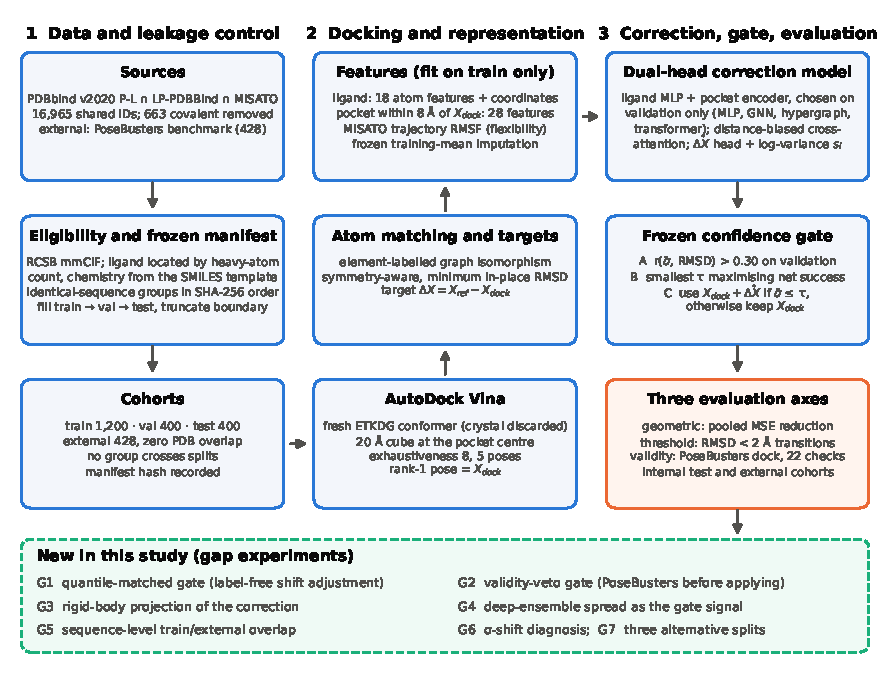
\includegraphics[width=\linewidth]{fig01_methodology.pdf}
\caption{Methodology. Column 1 builds the leakage-controlled cohorts, column 2 docks each complex and builds its
representation, column 3 trains the dual-head correction model, applies the frozen confidence gate and evaluates every
pose on three axes. The band lists the new analyses G1--G7 (G8, the deformation analysis, is in Section~\ref{sec:results}).}
\label{fig:method}
\end{figure}

\subsection{Datasets and eligibility}
\paragraph{Internal pool.} The PDBbind\,v2020 P-L set (19{,}443 complexes, as distributed in LP-PDBBind) was intersected
with the MISATO MD identifier lists (train, validation and test files; 16{,}972 identifiers), giving \IntersectN{} shared
complexes (original study: 16{,}627). \CovalentN{} covalent complexes were excluded using the LP-PDBBind flag. Structures
were downloaded from the RCSB PDB \citep{berman2000pdb} as mmCIF. The crystal ligand was located as the single
non-polymer residue whose heavy-atom count equals that of the LP-PDBBind SMILES and whose coordinates admit the SMILES
bond orders (RDKit \texttt{AssignBondOrdersFromTemplate}); the ligand was then sanitised with RDKit. Ligands spanning
several residues (mostly peptides) cannot be located this way and were excluded (\LigNotLocated{} complexes), as were
\StructFail{} entries whose structures failed to parse. The receptor retains polymer residues, metal ions and organic
cofactors, and drops water, common crystallisation additives, hydrogens, the ligand, and any hetero group within
1\,\AA{} of a ligand atom (alternate ligand copies).

\paragraph{External cohort.} The 428-complex PoseBusters benchmark set \citep{buttenschoen2024posebusters}, with its
supplied receptor and ligand files. Internal--external PDB-identifier overlap is zero.

\paragraph{Leakage-controlled manifest.} Complexes were grouped by identical protein sequence (LP-PDBBind chain
sequence). Groups were ordered by the SHA-256 digest of the group identifier and used to fill the training (1{,}200),
validation (400) and internal-test (400) splits in that order; only the boundary group is truncated and its unselected
members retired. Eligibility was checked before a complex took a slot. The manifest (SHA-256 recorded) was frozen before
any modelling. No group crosses splits.

\subsection{Docking and atom matching}
For each complex a fresh conformer was generated from the ligand graph with ETKDG and MMFF94 optimisation
\citep{riniker2015etkdg,halgren1996mmff}, discarding the crystal coordinates, and prepared with Meeko. Receptors were
converted to PDBQT with Open Babel \citep{oboyle2011openbabel}; receptor atoms of types Vina cannot score were removed.
AutoDock Vina was run with a 20\,\AA{} cubic box at the crystal-ligand centroid (pocket-informed), exhaustiveness 8, five
poses and a fixed seed; the rank-1 pose is the baseline $X_{dock}$. Docked and reference heavy atoms were matched by
element-labelled graph isomorphism, choosing among graph automorphisms the correspondence with the smallest in-place
RMSD (symmetry-corrected RMSD, no superposition). Complexes whose graphs did not match were excluded.

\subsection{Pocket representation and MISATO flexibility}
The pocket is the set of residues with any heavy atom within 8\,\AA{} of a docked ligand heavy atom, so it is defined
from the docked pose alone. Each residue node has 28 features: a 20-way amino-acid one-hot encoding, the C$\alpha$
position and side-chain-centroid offset relative to the docked-ligand centroid, a local degree (C$\alpha$ neighbours
within 10\,\AA{}), and a flexibility value. Ligand atoms carry 18 chemistry features (element, degree, aromaticity,
ring membership, formal charge, hydrogen count, hybridisation) and their coordinates. Edges link C$\alpha$ pairs
within 10\,\AA{}; hyperedges are chain segments of consecutive residues.

Flexibility is the per-residue root-mean-square fluctuation (RMSF) of the MISATO trajectory. Because the 133\,GB MISATO
file could not be stored, each complex's trajectory (100 frames) was read remotely by HTTP range requests. MISATO
coordinates are expressed in a different frame and residue numbering, so frame~0 was registered onto the crystal by
matching the ligand's heavy-atom graph (element-labelled isomorphism) and a Kabsch fit \citep{kabsch1976}; frames were
aligned on protein heavy atoms before computing per-atom RMSF, and each pocket residue receives the mean RMSF of MISATO
atoms within 1.5\,\AA{} of its heavy atoms. Registrations with ligand RMSD above 2\,\AA{} or median protein
nearest-neighbour distance above 2.5\,\AA{} were rejected. Residues without a mapped atom, complexes with rejected
registrations, and all external complexes receive the frozen training-set mean, the original study's prespecified
imputation rule. Continuous features and the coordinate scale were fitted on training complexes only.

\subsection{Correction model and uncertainty}
For $N$ matched atoms the target is $\Delta X = X_{ref} - X_{dock}$, the model predicts
$\hat{\Delta X} = f_\theta(X_{dock}, G_{pocket})$, and the corrected pose is $X_{corr} = X_{dock} + \hat{\Delta X}$.
The common architecture has a ligand MLP encoder, a pocket encoder, distance-biased cross-attention from ligand atoms to
pocket residues, a three-coordinate correction head and a per-atom log-variance head $s_i$ (clamped to $[-12,12]$), with
$\sigma_i = \exp(s_i/2)$. The training objective is the heteroscedastic negative log-likelihood
\begin{equation}
\mathcal{L}_{NLL} = \tfrac{1}{2}\,\mathrm{mean}_i\!\left[3 s_i + \lVert \hat{\Delta X}_i - \Delta X_i \rVert_2^2 / e^{s_i}\right].
\end{equation}
The four candidate pocket encoders are an MLP over residue features, a distance-weighted message-passing GNN
\citep{gilmer2017mpnn}, a residue-incidence hypergraph encoder with flexibility-weighted segment attention, and a
transformer with a learned distance bias. All use hidden size 64 and two encoder layers, and are trained with Adam
(learning rate $10^{-3}$), at most 15 epochs and patience 5 on validation NLL, with random proper rotations of all
coordinates and targets during training only. Five seeds (0, 42, 123, 999, 2026) were trained per architecture; the
architecture with the highest mean validation pooled MSE reduction was selected. Held-out data were not used for
selection.

\subsection{Confidence gate}
Let $\bar\sigma_j$ be the mean predicted $\sigma$ of seed--complex row $j$. Stage~A requires the pooled validation Pearson
correlation between $\bar\sigma$ and baseline RMSD to exceed 0.30. Stage~B sweeps every distinct validation $\bar\sigma$
and selects the smallest threshold maximising pooled validation net success,
\begin{equation}
\tau = \min\{t : \mathrm{NetSuccess}(t) = \max_{t'} \mathrm{NetSuccess}(t')\},
\end{equation}
where NetSuccess is the RMSD\,$<$\,2\,\AA{} success rate when the correction is applied to rows with $\bar\sigma_j \le t$
minus the baseline success rate. Stage~C applies the frozen $\tau$ to held-out data without adjustment.

\subsection{Evaluation}
\emph{Geometric:} pooled MSE reduction $100\,(\mathrm{MSD}_{base}-\mathrm{MSD}_{corr})/\mathrm{MSD}_{base}$ over all atoms.
\emph{Threshold:} success is RMSD\,$<$\,2\,\AA{}; transitions are preservation (success$\to$success), harm (success$\to$failure),
rescue (failure$\to$success) and persistent failure. \emph{Validity:} the full PoseBusters \texttt{dock} configuration
(22 binary checks: loading, sanitisation, InChI, connectivity, radicals, bond lengths and angles, internal clash, ring
and double-bond flatness, internal energy, and protein-ligand distance and volume-overlap checks), applied to heavy-atom
poses against the receptor; a pose is valid only if every check passes, and a check not computed after an upstream
failure counts as failed. Gated poses are the corrected pose when the gate fires, otherwise the baseline. Uncertainty
intervals are reported in two ways: a Student-$t$ interval over the five seed-level rates, and a 10{,}000-resample paired
complex-level percentile bootstrap.

\paragraph{Statistical validation.} A training-only permutation test relates each atom's distance to the nearest pocket
C$\alpha$ to its target displacement magnitude, shuffling magnitudes within complexes (10{,}000 permutations). A rotational
audit compares predictions before and after a random rotation (rotated back) for ten validation complexes and five seeds.
A synthetic identity check verifies $\mathrm{RMSE}_{component} = \mathrm{RMSD}/\sqrt{3}$.

\subsection{New analyses (G1--G7)}\label{sec:gaps}
\begin{description}
\item[G1 Quantile-matched gate.] The validation admit fraction $q$ is frozen; each held-out cohort is gated at the
      $q$-quantile of its own $\bar\sigma$ distribution. No held-out label is used. This tests whether matching the admit
      rate, rather than the absolute threshold, removes the effect of uncertainty-scale shift.
\item[G2 Validity veto.] A correction is applied only if the corrected pose passes all PoseBusters checks (alone, and
      combined with the $\sigma$ gate). PoseBusters needs only the pose and receptor, so the rule is deployable.
\item[G3 Rigid-body projection.] The free per-atom correction is replaced by the rigid motion of the docked pose that
      best fits it (Kabsch). Internal geometry is preserved by construction; the gate is recalibrated on validation with
      the same rule.
\item[G4 Deep-ensemble uncertainty.] The five seeds' mean correction is gated by their spread (mean per-atom standard
      deviation), calibrated exactly as in Stage~B; a rigid-projected variant is also evaluated.
\item[G5 Sequence-level leakage.] Exact and near-identical (3-mer Jaccard $\ge$ 0.9) chain-sequence overlap between the
      training set and the external cohort, and outcomes stratified by overlap.
\item[G6 Uncertainty-shift diagnosis.] Per-cohort $\bar\sigma$ distributions (two-sample Kolmogorov--Smirnov tests),
      $\sigma$--RMSD correlation per cohort, and cohort descriptors (ligand size, pocket size).
\item[G7 Split variance.] The docked internal pool is re-partitioned three times with the same group-aware rule and
      different hash salts; the selected architecture is retrained (five seeds each) and re-evaluated.
\end{description}

\subsection{Deviations from the original protocol}\label{sec:deviations}
\begin{itemize}
\item \emph{Structures:} PDBbind's curated files require registration, so structures came from the RCSB PDB and ligand
      chemistry from LP-PDBBind SMILES. Multi-residue ligands were excluded (the original study excluded none for this
      reason).
\item \emph{Grouping:} identical protein sequence was used as the leakage group; the original used LP-PDBBind grouping
      (1{,}792 candidate-touching groups versus \TouchedGroups{} here).
\item \emph{Software:} AutoDock Vina 1.2.7 (original: 1.2.0), RDKit 2026.09, PoseBusters 0.6.5.
\item \emph{Docked-pose export:} Meeko's RDKit export was used instead of an Open Babel PDBQT$\to$SDF conversion; the
      Open Babel conversion of the same pose was retained to test the conversion artifact reported in the original study.
\item \emph{Flexibility:} MISATO RMSF obtained through the registration procedure above; the original's exact mapping
      was not specified.
\item \emph{Validity audit:} poses were audited as heavy-atom molecules for all variants, which avoids hydrogens being
      left behind by a heavy-atom correction.
\end{itemize}


\section{Results}\label{sec:results}

\subsection{Cohorts and docking baseline}
All \NInt{} internal-test and \NExt{} external complexes docked and matched (no atom-matching exclusions), giving
\RowsInt{} and \RowsExt{} seed--complex rows. Vina rank-1 success (RMSD\,$<$\,2\Ang) was \BaseInt\% internally and
\BaseExt\% externally, against 55.6\% and 60.7\% in the original study (Table~\ref{tab:compare}). The internal gap is the
largest difference in inputs between the two studies and is consistent with the use of RCSB rather than PDBbind-prepared
structures; mean baseline RMSD was \BaseRMSDVal{}, \BaseRMSDInt{} and \BaseRMSDExt\Ang{} for validation, internal test and
external.

\subsection{Architecture selection}
On validation only, the four encoders reached almost identical pooled MSE reductions (Fig.~\ref{fig:selection}):
MLP \SelMLP\%, GNN \SelGNN\%, hypergraph \SelHypergraph\% and transformer \SelTransformer\%. The transformer had the highest
mean and was selected; paired seed-level $t$-tests favoured it over each alternative (MLP $p=\PMLP$, GNN $p=\PGNN$,
hypergraph $p=\PHypergraph$), but the one-way ANOVA across all four was not significant ($F=\AnovaF$, $p=\AnovaP$). The
original study selected the MLP. In both studies the spread between encoders is under one percentage point, so the choice of
encoder is not what drives the outcomes below.

\begin{figure}[H]
\centering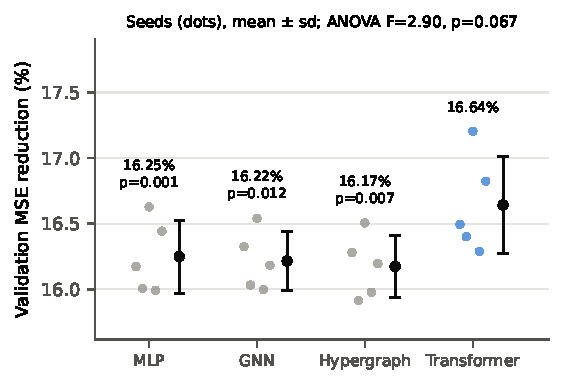
\includegraphics[width=0.62\linewidth]{fig02_selection.pdf}
\caption{Validation-only architecture selection: mean pooled MSE reduction over five seeds (dots: seeds).}
\label{fig:selection}
\end{figure}

\subsection{Statistical validation}
The training-only permutation test (\PermComplexes{} complexes, \PermAtoms{} heavy atoms, 10{,}000 permutations) depends on
how ``pocket distance'' is defined, which the original study did not specify. Using the distance from each atom to the pocket
centroid, the correlation with target displacement was $r=\PermRCen$ against a within-complex null mean of \PermNullCen{}
($p=\PermPCen$, two-sided around the null mean). Using the distance to the nearest pocket C$\alpha$, it was $r=\PermRCa$,
significantly \emph{below} its null mean of \PermNullCa{} ($p=\PermPCa$). Because within-complex shuffling preserves the
between-complex association, the null is not centred at zero; a test that compares $|r|$ against $|r_{null}|$ would report
$p=1$ for the second definition. The rotational audit (50 observations) gave a mean prediction discrepancy of \RotMean\Ang{}
(median \RotMedian, 95th percentile \RotPct, maximum \RotMax\Ang), confirming that the cross-attention model is not rotation
equivariant (original: 0.53\Ang{} mean). The metric identity held to \MetricId.

\subsection{RMSD-threshold outcomes}
Ungated correction reduced pooled MSE by \MSEInt\% internally (seed range \MSEIntMin--\MSEIntMax\%) and \MSEExt\% externally
(\MSEExtMin--\MSEExtMax\%), but it lowered success from \BaseInt\% to \SuccUngInt\% internally (\NetUngInt{}\,pp; bootstrap
95\% CI [\BootUngIntLo, \BootUngIntHi]) and from \BaseExt\% to \SuccUngExt\% externally (\NetUngExt{}\,pp; CI
[\BootUngExtLo, \BootUngExtHi]; Fig.~\ref{fig:rmsd}). Both decreases are significant and much larger than the original
internal decrease ($-3.6$\,pp), and the original external change was null. Harm dominated rescue among the transitions
(Fig.~\ref{fig:transitions}): internally \TrUngIntHarm{} harmed versus \TrUngIntRescue{} rescued rows, externally
\TrUngExtHarm{} versus \TrUngExtRescue.

\begin{figure}[H]
\centering
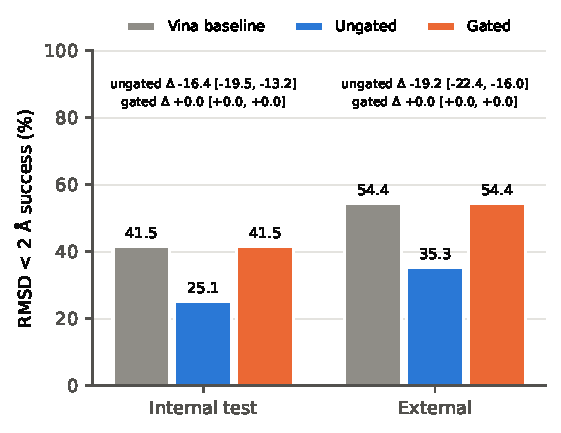
\includegraphics[width=0.48\linewidth]{fig04_rmsd_success.pdf}\hfill
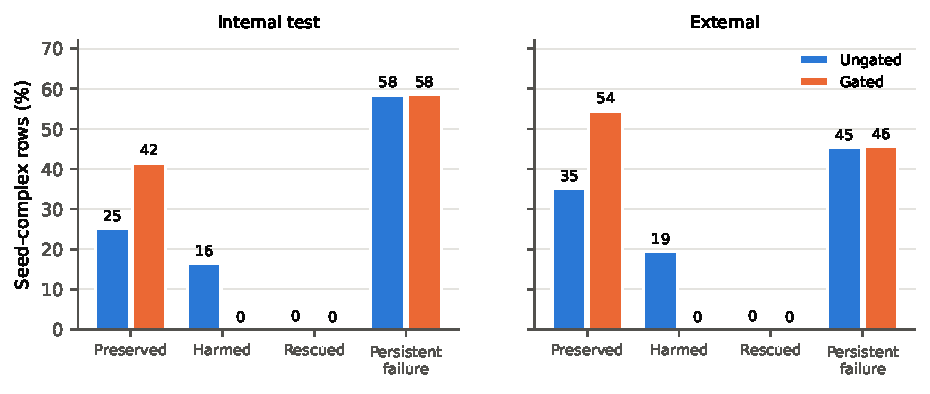
\includegraphics[width=0.5\linewidth]{fig03_transitions.pdf}
\caption{Left: RMSD\,$<$\,2\Ang{} success of the Vina baseline, ungated and gated correction, with net change and
bootstrap 95\% CI. Right: transition classes (share of seed--complex rows).}
\label{fig:rmsd}\label{fig:transitions}
\end{figure}

\subsection{Confidence gate}
Stage~A passed narrowly: the validation correlation between mean $\sigma$ and baseline RMSD was \StageA{} (threshold 0.30).
Stage~B selected $\tau=\Tau\Ang$, the smallest threshold reaching the maximum validation net success of \ValNet\,pp---the
same value the original study reported---but this threshold admits only \AdmitVal\% of validation rows, \AdmitInt\% of
internal-test rows and \AdmitExt\% of external rows (original: 24.15\%, 23.4\% and 55.5\%). The gated system is therefore
almost identical to the baseline: gated success equalled baseline success in both cohorts (net \NetGatInt{} and
\NetGatExt\,pp). The baseline-RMSD control gate reproduced the original observation that no ``correct only good poses''
threshold helps (best net \CtrlLe\,pp), but the opposite rule---correct only poses with baseline RMSD $\ge$\,\CtrlGeT\Ang---
reached \CtrlGe\,pp on validation, so on this split a baseline-quality signal (if it were available at inference) would
outperform the learned uncertainty.

\subsection{Chemical validity}
Baseline poses passed all 22 PoseBusters checks in \PassBaseInt\% (internal) and \PassBaseExt\% (external) of rows. After
ungated correction only \PassUngInt\% and \PassUngExt\% passed (Fig.~\ref{fig:validity}); among rows with a valid baseline,
\NewInvUngInt\% and \NewInvUngExt\% became invalid. The gate kept \PassGatInt\% and \PassGatExt\% valid (newly invalid:
\NewInvGatInt\% and \NewInvGatExt\%; relative reduction \RelRedInt\% and \RelRedExt\%), but only because it rarely fired.
Validity loss was independent of the RMSD transition class: even among \emph{preserved} rows, \InvIntPreservation\% (internal)
and \InvExtPreservation\% (external) of corrected poses were invalid (Fig.~\ref{fig:cross}). The failing checks were
intramolecular (Fig.~\ref{fig:checks}): bond lengths (\ChkIntBondlengths\% of corrected internal poses), bond angles
(\ChkIntBondangles\%), internal steric clash (\ChkIntInternalstericclash\%) and internal energy (\ChkIntInternalenergy\%);
protein-distance failures were far less common (\ChkIntMinimumdistancetoprotein\%). Among \SpotN{} preserved-but-invalid
internal poses (seed 0) the shortest bond shrank to a median \SpotBondMed\% of its docked length (minimum \SpotBondMin\%),
and bond angles changed by up to \SpotAngleMax$^\circ$.

\begin{figure}[H]
\centering
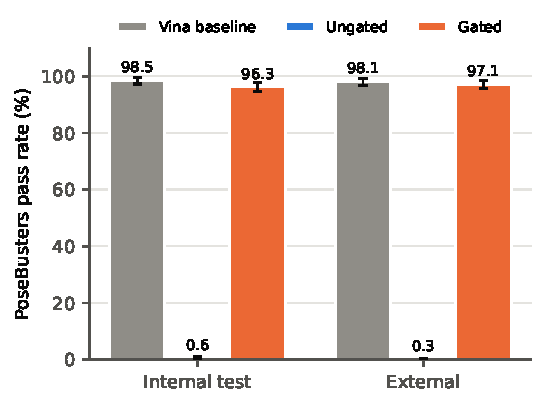
\includegraphics[width=0.48\linewidth]{fig05_posebusters_pass.pdf}\hfill
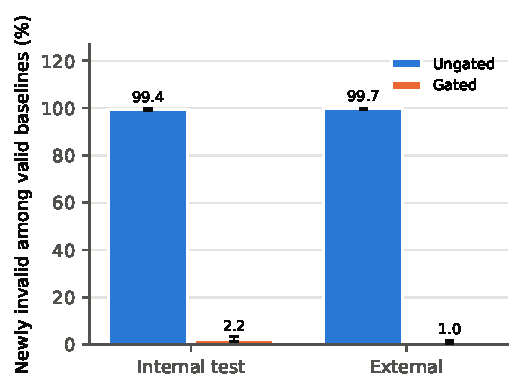
\includegraphics[width=0.48\linewidth]{fig06_newly_invalid.pdf}
\caption{Left: PoseBusters pass rate (bootstrap 95\% CI). Right: rate at which correction invalidates a valid baseline.}
\label{fig:validity}
\end{figure}

\begin{figure}[H]
\centering
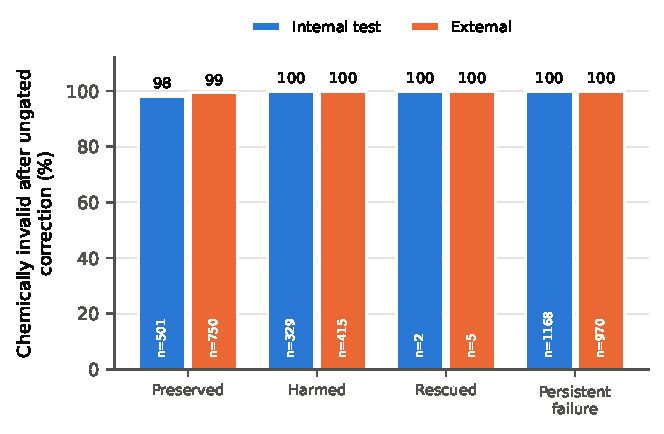
\includegraphics[width=0.52\linewidth]{fig07_invalid_by_transition.pdf}\hfill
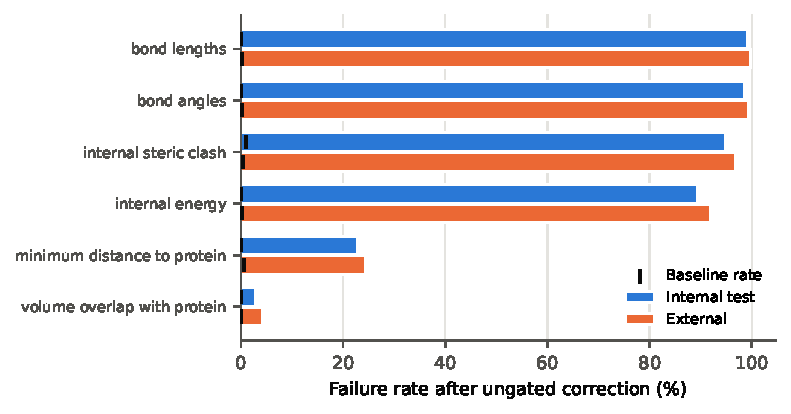
\includegraphics[width=0.46\linewidth]{fig08_check_failures.pdf}
\caption{Left: invalidity of corrected poses within each RMSD transition class. Right: failure rate of each PoseBusters
check after ungated correction (bars) against the baseline (ticks); checks below 1\% are omitted.}
\label{fig:cross}\label{fig:checks}
\end{figure}

\paragraph{The conversion artifact} The original study traced many baseline sanitisation failures to nitrogen atoms with
valence four and no formal charge introduced by PDBQT$\to$SDF conversion. Converting the same rank-1 poses with Open Babel
reproduced it: \ObabelInt{} internal-test complexes (\ObabelAtomsInt{} such atoms) and \ObabelExt{} external complexes failed
sanitisation, close to the original 150 and 4. Meeko's export, used for all analyses here, does not produce the artifact, so
no repair was needed.

\subsection{Why correction destroys chemistry (G3, G8)}
Every predicted correction was decomposed into the rigid motion that best maps the docked pose onto the corrected pose and a
residual internal deformation. The internal part made up a median \InternalShareInt\% (internal) and \InternalShareExt\%
(external) of the correction's squared magnitude. Corrected ligands contracted to a median \RgCorrInt{} (interquartile range
\RgCorrIntLo--\RgCorrIntHi) and \RgCorrExt{} of their docked radius of gyration, and \ContractedInt\% of internal rows shrank
below 0.8, whereas crystal poses keep the docked size (median ratio \RgRefInt; Fig.~\ref{fig:shrink}a). When the correction
was replaced by its rigid part (G3), validity was largely preserved (\PassRigidInt\% and \PassRigidExt\% passed), but the error
reduction vanished (\GrMSEInt\% and \GrMSEExt\%), and the recalibrated gate admitted nothing. The pooled error reduction is
therefore produced by contracting the ligand, not by moving it towards the crystal pose.

Pooled MSE also hides who benefits. Contraction reduces the error of badly docked poses, whose atoms are far from the
reference in all directions, but increases it for good poses (Fig.~\ref{fig:shrink}b). The median per-complex change in squared
error was \MedianGainInt\% internally and \MedianGainExt\% externally---an \emph{increase}---while the pooled reduction was
positive because a minority of high-error complexes dominates the pooled sum.

\begin{figure}[H]
\centering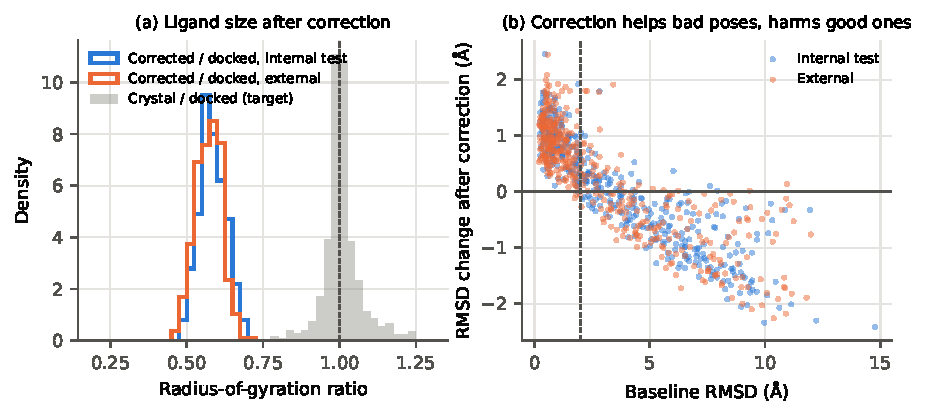
\includegraphics[width=\linewidth]{fig12_shrinkage.pdf}
\caption{(a) Radius-of-gyration ratio of corrected to docked ligands (lines) and of crystal to docked ligands (shaded).
(b) RMSD change after correction against baseline RMSD (seed 0); dashed line: 2\Ang.}
\label{fig:shrink}
\end{figure}

\subsection{Alternative decision rules (G1, G2, G4)}
None of the label-free decision rules produced a positive held-out success change (Fig.~\ref{fig:gates}). The quantile-matched
gate (G1) fixed the admit fraction at the validation value (\GqQ\%) in each cohort, removing the absolute-scale dependence, but
success did not change (net \GqGNetInt{} and \GqGNetExt\,pp) and external validity fell slightly (\GqPassGatExt\% against \GzPassGatExt\% for the frozen gate). The validity veto (G2) is
deployable---PoseBusters needs no ground truth---but almost no corrected pose passed it (admit \VetoAdmitInt\% and
\VetoAdmitExt\%), so it reduces to ``never correct''. The five-seed ensemble (G4) reduced pooled MSE slightly more than single
models (\GeMSEInt\% and \GeMSEExt\%) and its spread correlated with baseline RMSD ($r=\GeStageA$, below the 0.30 Stage~A
threshold), but averaging five contracting predictions produced invalid poses throughout (\PassEnsInt\% valid). A rigid
ensemble kept validity (\PassEnsRigidInt\%) with negligible geometric effect.

\begin{figure}[H]
\centering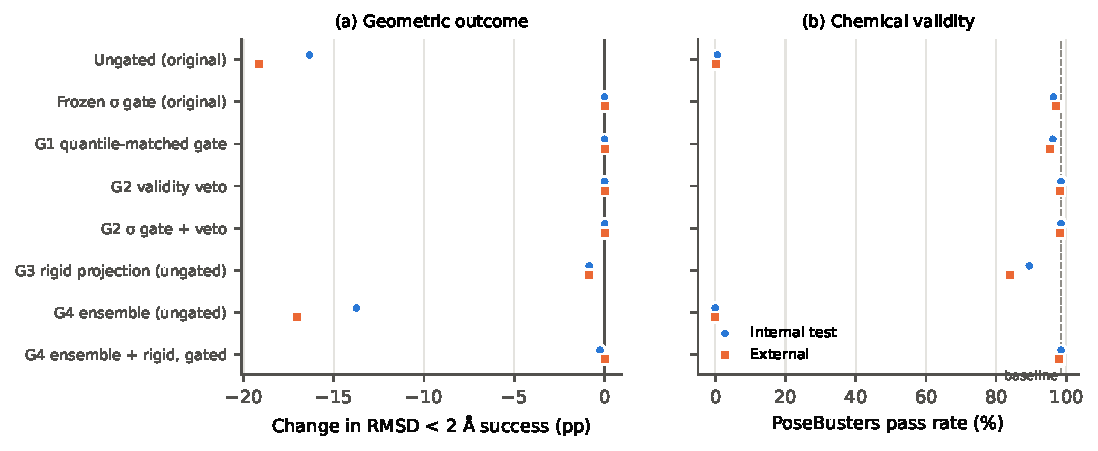
\includegraphics[width=\linewidth]{fig09_gate_variants.pdf}
\caption{Held-out success change against PoseBusters pass rate for the original gate and the new decision rules.}
\label{fig:gates}
\end{figure}

\subsection{Sequence-level leakage (G5)}
Although no PDB identifier is shared, \SeqExact{} external complexes contain a protein chain identical to a training chain and
\SeqNear{} (\SeqNearPct\%) are near-identical (3-mer Jaccard $\ge$\,0.9). On these \SeqNearN{} complexes ungated correction
reduced pooled MSE by \SeqNearMSE\%, against \SeqNovelMSE\% on the \SeqNovelN{} novel ones; RMSD-threshold harm was large in
both groups (\SeqNearNet{} and \SeqNovelNet\,pp). PDB-identifier disjointness therefore overstates how ``external'' the
PoseBusters cohort is for a PDBbind-trained model, and the external error reduction is concentrated on familiar proteins.

\subsection{Uncertainty shift (G6)}
The original study attributed weaker external gating to predicted $\sigma$ being about 32\% lower externally. Here the mean
external $\sigma$ differed from validation by only \SigShiftExt\% (Kolmogorov--Smirnov $D=\KSExtD$, $p=\KSExtP$), while the
internal test differed by \SigShiftInt\% ($D=\KSIntD$). The $\sigma$--RMSD correlation fell from \SigRVal{} (validation) to
\SigRInt{} (internal) and \SigRExt{} (external), and $\sigma$ was essentially unrelated to the per-complex benefit of
correcting (Spearman \SigGainVal, \SigGainInt, \SigGainExt). The gate fails here not because $\sigma$ shifts but because it
ranks poses by how wrong they are, not by whether correcting them helps (Fig.~\ref{fig:sigma}).

\begin{figure}[H]
\centering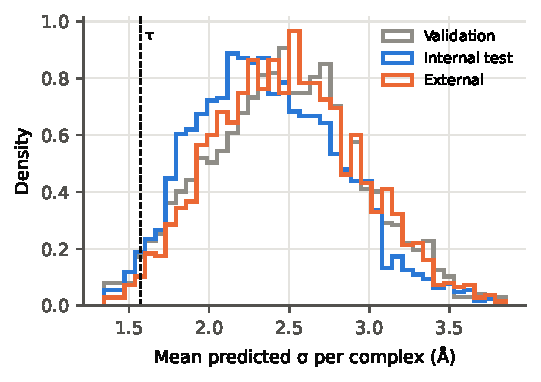
\includegraphics[width=0.6\linewidth]{fig10_sigma_shift.pdf}
\caption{Distribution of mean predicted $\sigma$ per complex by cohort; dashed line: frozen threshold $\tau$.}
\label{fig:sigma}
\end{figure}

\subsection{Split-to-split variance (G7)}
Re-partitioning the internal pool three times with the same group-aware rule (Fig.~\ref{fig:splits}) left the main pattern
intact: internal MSE reductions of \SAMSEInt, \SBMSEInt{} and \SCMSEInt\%, success changes of \SANetInt, \SBNetInt{} and
\SCNetInt\,pp, and ungated validity below 1\%. The gate, however, depends on the split: Stage~A \SAPass{} ($r=\SAStageA$),
\SBPass{} ($r=\SBStageA$) and \SCPass{} ($r=\SCStageA$) on the three alternatives, so on every alternative split no gate would
have been deployed at all.

\begin{figure}[H]
\centering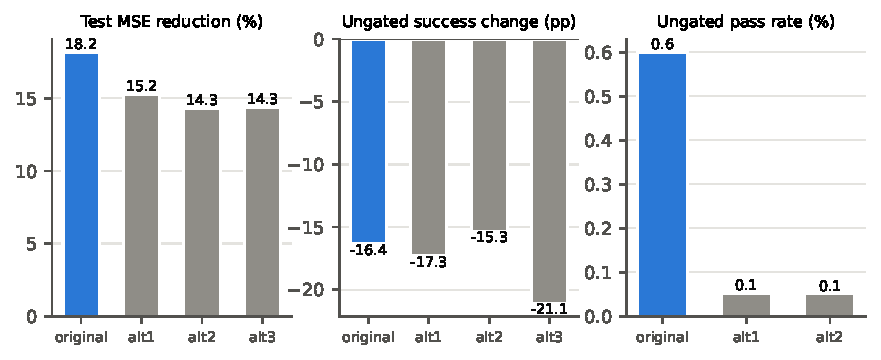
\includegraphics[width=\linewidth]{fig11_split_variance.pdf}
\caption{Original split and three alternative group-aware splits.}
\label{fig:splits}
\end{figure}

\subsection{Comparison with the original study}
\begin{table}[H]
\centering\small
\caption{Headline results of the original study and of this reproduction (internal\,/\,external where two values are given).}
\label{tab:compare}
\begin{tabular}{@{}p{5.3cm}p{3.1cm}p{3.6cm}l@{}}
\toprule
Quantity & Original & Reproduction & Verdict \\
\midrule
ID intersection & 16{,}627 & \IntersectN & \ok \\
Covalent exclusions & 651 & \CovalentN & \ok \\
Vina success (\%) & 55.6 / 60.7 & \BaseInt{} / \BaseExt & \partly \\
Selected encoder & MLP ($p_{\text{ANOVA}}=0.010$) & \SelArch{} ($p_{\text{ANOVA}}=\AnovaP$) & \no \\
Pooled MSE reduction (\%) & 9.75 / 11.35 & \MSEInt{} / \MSEExt & \ok \\
Ungated success change (pp) & $-3.6$ / n.s. & \NetUngInt{} / \NetUngExt & \partly \\
Gate val.\ net success (pp) & +0.10 & +\ValNet & \ok \\
Gate admit rate val / int / ext (\%) & 24.2 / 23.4 / 55.5 & \AdmitVal{} / \AdmitInt{} / \AdmitExt & \no \\
External vs.\ validation $\sigma$ & $-32\%$ & \SigShiftExt\% & \no \\
PoseBusters pass, baseline (\%) & 96.45 / 97.66 & \PassBaseInt{} / \PassBaseExt & \ok \\
PoseBusters pass, ungated (\%) & 31.22 / 59.02 & \PassUngInt{} / \PassUngExt & \partly \\
PoseBusters pass, gated (\%) & 89.04 / 83.64 & \PassGatInt{} / \PassGatExt & \partly \\
Newly invalid, ungated (\%) & 67.6 / 39.9 & \NewInvUngInt{} / \NewInvUngExt & \partly \\
Invalid within preserved class (\%) & 70.1 / 34.8 & \InvIntPreservation{} / \InvExtPreservation & \partly \\
Permutation $r$ & 0.51 & \PermRCen{} (centroid) & \partly \\
Rotation discrepancy, mean (\AA) & 0.53 & \RotMean & \ok \\
Open Babel artifact (complexes) & 150 / 4 & \ObabelInt{} / \ObabelExt & \ok \\
\bottomrule
\end{tabular}
\end{table}
\noindent ``Partly'' marks results with the same direction and conclusion but a clearly different magnitude.

\section{Discussion}\label{sec:discussion}

\paragraph{Interpretation of findings} The reproduction confirms the qualitative claims of the original study---continuous
error falls while RMSD-threshold success and chemical validity fall with it---and shows that the effect is stronger and has a
simple cause. The learned correction mostly contracts the ligand. Contraction lowers squared error for badly docked poses and
for the pooled metric, but it breaks bonds and angles in nearly every pose and moves good poses out of tolerance.

\paragraph{Relation to the research questions} For Q1, the data pipeline, docking baseline, metric behaviour, rotation audit
and conversion artifact reproduced closely; the selected encoder, the size of the RMSD harm, the gate's operating point and
the uncertainty-shift explanation did not (Table~\ref{tab:compare}). For Q2, measuring the gaps was more productive than
closing them: none of the label-free decision rules made correction beneficial, but the analyses located the failure in the
correction itself rather than in the gate.

\paragraph{Relation to prior work} PoseBusters showed that learned docking can satisfy RMSD criteria with invalid chemistry
\citep{buttenschoen2024posebusters}; the original study extended this to post-hoc correction
\citep{mwamughunda2026original}. Our results add the mechanism: the conditional mean of atom positions under pose uncertainty
lies inside the molecule, so a model trained with squared error (or a Gaussian likelihood, which shares its mean) learns to
predict a contracted pose. This mirrors the regression-to-the-mean blurring familiar from deterministic structure predictors
and is one reason generative docking methods sample poses instead of regressing them \citep{corso2023diffdock}. The external
sequence overlap agrees with PoseBusters' observation that performance depends on similarity to the training proteins.

\paragraph{Explanation of unexpected results} Three differences from the original need explanation. First, the harm is larger
here, plausibly because our docking baseline is worse (larger targets, more contraction) and because our encoder choice was
not the original MLP; the effect persisted across all four encoders and three alternative splits, so it is not an artefact of
one model. Second, the gate admitted almost nothing: with stronger harm, the validation net-success curve peaks at a very low
admit fraction. Third, the uncertainty did not shrink externally, so the original explanation of weaker external gating does
not transfer; the deeper problem is that $\sigma$ tracks how wrong a pose is, not whether correcting it helps.

\paragraph{Theoretical implications} Evaluating refinement by pooled MSE rewards contraction. A refinement objective should
be defined over chemically valid poses---rigid-body motions, torsions, or a learned distribution over conformers---so that the
optimum cannot leave the space of molecules. The decomposition into rigid and internal parts is a simple diagnostic that any
coordinate-regression model can report.

\paragraph{Practical implications} For practitioners, a learned per-atom correction of this kind should not be applied to
docking output without a validity check, and a validity veto is cheap and deployable. Gating on predicted uncertainty is not
enough: on every alternative split the gate failed its own correlation check, and on the original split it chose to correct
almost nothing. Reports of
external performance should include sequence-level similarity to the training data, not only identifier overlap.

\paragraph{Limitations} Structures came from the RCSB PDB because PDBbind's curated files require registration; multi-residue
ligands were therefore excluded and the internal docking baseline is weaker than in the original study. MISATO flexibility was
mapped through our own registration because the original mapping was not specified. We ran one correction family (the original
architecture and objective); other objectives may behave differently. Audits were performed on heavy-atom poses. Computing
resources were a 4-core CPU without GPU, so seeds and splits were limited to those reported.

\paragraph{Future research} Natural next steps are correction models constrained to rigid and torsional motions, objectives
that penalise bond-length and angle deviations, generative refinement that samples rather than averages, and gates trained
directly on the per-complex benefit of correcting rather than on predicted error.

\section{Conclusion}\label{sec:conclusion}
Learned post-docking correction promises to fix docking errors, but an earlier study warned that it can also break poses and
chemistry, and that a confidence gate only partly helps. We rebuilt that study independently from public data to test its
claims and the gaps it left open.

The main warnings hold, and more strongly. Applying the correction to every pose lowered pooled coordinate error but reduced
docking success by about 16--19 percentage points and left fewer than 1\% of poses chemically valid.

Our new analyses show why. The model learns to shrink each ligand towards its centre: this lowers the average error, because
a few badly docked poses dominate it, but distorts bonds and harms good poses. Moving the ligand only as a rigid body keeps the
chemistry valid but removes the benefit.

The confidence gate did not solve this. It rarely corrected anything, failed its own check on all three alternative splits,
and the reported uncertainty shift under distribution change did not reproduce.

The takeaway is that pose refinement should be judged per complex, on validity as well as geometry, and built so that it can
only produce real molecules.

\section*{Data and code availability}
All code, the frozen manifest and its hash, every result file and the scripts that regenerate each number (\texttt{numbers.tex})
and figure in this paper are in the \texttt{DockingPoseCorrection} folder of the accompanying repository. Source data are public:
LP-PDBBind, the MISATO identifier lists and trajectories (Zenodo record 7711953), the RCSB PDB, and the PoseBusters benchmark
(Zenodo record 8278563).

\section*{Declaration of generative AI use}
The authors used an AI coding assistant (Claude, Anthropic) to implement the reproduction pipeline, run the experiments and draft
the manuscript. The authors reviewed and are responsible for all content.

\section*{Declaration of competing interest}
The authors declare no competing interests.

\bibliographystyle{elsarticle-harv}
\bibliography{refs}
\end{document}
